\chapter{SP2-CU18 Eliminar subrayado en sección de propuesta de Unidad de Aprendizaje}
\begin{UseCase}{SP2-CU18}{ Eliminar subrayado en sección de propuesta de Unidad de Aprendizaje }{El usuario podrá eliminar el subrayado especifico en el texto previamente realizados en la sección de propuesta de Unidad de Aprendizaje que se está revisando.}
		\UCitem{Versión}{\color{Gray}1.0}
		\UCitem{Autor}{\color{Gray}Romero Ponce Mauricio Isaac}
		\UCitem{Supervisa}{\color{Gray}Parra Garcilazo Cinthya Dolores}
		\UCitem{Actor}{Analista}
		\UCitem{Propósito}{Quitar resaltados no relevantes en el texto.}
		\UCitem{Entradas}{}
		\UCitem{Origen}{Mouse.}
		\UCitem{Salidas}{
      \hypertarget{CU18-MSG13}{
      \begin{itemize}
        \item MSG13 Error interno: Intentelo más tarde.
      \end{itemize}
        }
                    }
		\UCitem{Destino}{Pantalla.}
		\UCitem{Precondiciones}{ Se llamó al caso de uso SP2-CU17}
		\UCitem{Postcondiciones}{
            \begin{itemize}
                \item Se eliminará del sistema el resaltado en la sección del documento.
                \item Desaparecerá de la vizualización del texto el resaltado.  
             \end{itemize}  
        }
		\UCitem{Errores}{}
		\UCitem{Estado}{Revisión.}
		\UCitem{Observaciones}{}
\end{UseCase}

%--------------------------- CU TRAYECTORIA PRINCIPAL -------------------------
\begin{UCtrayectoria}{Principal}


    \UCpaso[\UCactor] Presiona el botón \IUbutton{Eliminar subrayado}. 
    
    \UCpaso Elimina el resaltado en la sección del documento del sistema. \hyperref[SP2-CU18-A]{Trayectoria A}.
\end{UCtrayectoria}

%------------------------ CU TRAYECTORIA ALTERNARIVA A -------------------------

\label{SP2-CU18-A}
\begin{UCtrayectoriaA}{A}{No se pudo eliminar el comentario en el sistema}
  \UCpaso Muestra el mensaje \MSGref{CU16-MSG13}{Error interno: Intentelo más tarde}.
  \UCpaso[\UCactor] Cierra el mensaje presionando \IUbutton{Aceptar}.
\end{UCtrayectoriaA}


\chapter{Pantallas}
 \begin{figure}
  \centering
    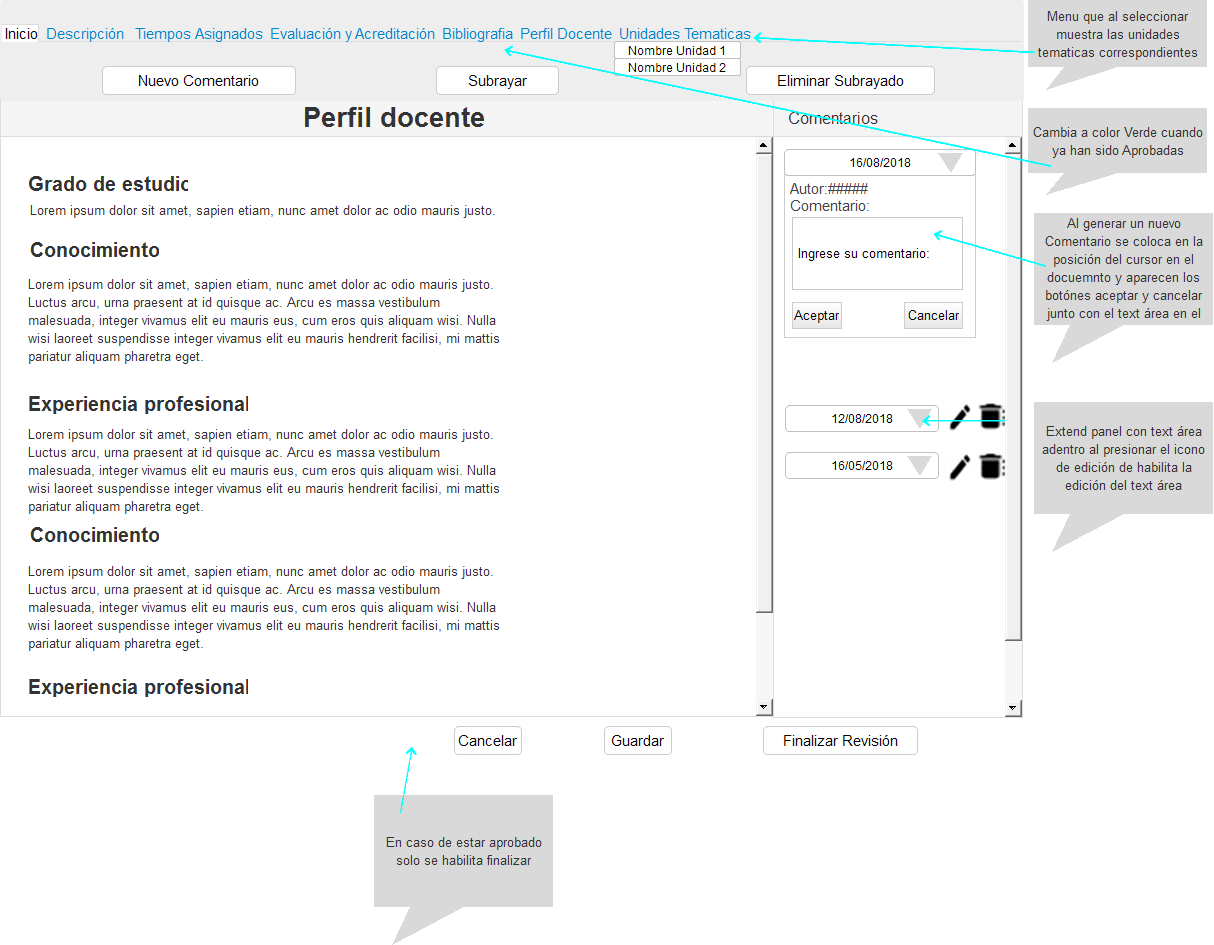
\includegraphics[width=0.7\textwidth]{DCU/SP2/Pantallas/Nuevo_comentario}
  \caption{SP2-IU-Nuevo comentario}
  \label{SP2-IU-Nuevo_comentario}
\end{figure}
